\section{Monte Carlo Validation on a Known-Truth DGP}
\label{app:mc-validation}

The HealthBench experiment in the body reports per-policy Mean and CVaR-CJE
estimates with calibration-aware confidence intervals and transport audits,
but on real data the ground truth is what it is and we cannot directly check
whether the CIs cover, what RMSE looks like at smaller oracle slices, or how
often each audit fires under controlled mis-specification. This appendix
addresses that gap: we fit a per-policy semi-synthetic data-generating
process to the HealthBench panel, sample new datasets from it, run the full
production pipeline (designed oracle slice, isotonic calibration, bootstrap
CI, jackknife $\Var_{\text{cal}}$, two-moment CVaR audit, mean transport
audit), and aggregate over Monte Carlo replicates to measure coverage,
RMSE, audit size at the null, and audit power under perturbation.

The full code lives at \texttt{cvar\_v4/eda/deeper/mc\_validation/}; the
estimator and audit machinery are reused unmodified from
\texttt{cvar\_v4/eda/deeper/\_estimator.py}.

\paragraph{Semi-synthetic DGP.}
For each of the six HealthBench policies $\pi \in \{\texttt{base},
\texttt{clone}, \texttt{premium}, \texttt{parallel\_universe\_prompt},
\texttt{unhelpful}, \texttt{risky}\}$ we fit a fully-parametric joint
$(\Sscore, \Y)$:
\begin{itemize}[leftmargin=*,nosep]
  \item $\Y$ is sampled from the empirical CDF of the policy's full-oracle
    labels. For policies with non-trivial mass at $\Y{=}0$
    (rubric-criterion blanket failures), the marginal is modeled as a
    mixture: $P(\Y{=}0)=p_{\text{zero}}$ and the conditional CDF on
    $\Y{>}0$ is the empirical CDF of the strictly-positive labels.
  \item $\Sscore \mid \Y$ is generated as $\hat m_\pi(\Y) + \sigma_\pi(\Y)\,\varepsilon$,
    clipped to $[0, 1]$, where $\hat m_\pi$ is an isotonic fit of $E[\Sscore \mid \Y]$
    and $\sigma_\pi(\Y)$ is heteroscedastic (4 bins by Y-quartile) with $\varepsilon \sim \mathcal{N}(0, 1)$.
  \item Cross-policy joint structure is \emph{not} preserved (policies are
    sampled independently). The estimator is per-policy in production, so
    only the per-policy marginals matter for inference.
\end{itemize}

\textit{Mis-specification knob.} We can swap in $\hat m_{\text{base}}$ as the
target's conditional mean (the well-specified null on $\hat m$) and add a
controlled shift $\delta$ either uniformly ($\hat m{+}\delta$) or only on
the lower tail $\Y{\le}q_{\alpha}(\Y_{\text{base}})$
($\hat m{-}\delta\cdot\ind{\Y\le q_\alpha}$).

\paragraph{Pipeline replicated per MC rep.}
For each cell $(\pi', n, \text{cov}, \alpha, \text{design}, \delta, \text{pert})$ and seed $b$:
\begin{enumerate}[leftmargin=*,nosep]
  \item Sample $n$ logger-policy and $n$ target-policy $(\Sscore, \Y)$ pairs from the DGP.
  \item Apply \texttt{select\_slice} to the logger panel to get
    $(\Sscore_{\text{train}}, \Y_{\text{train}}, w_{\text{train}}{=}1/\pi)$
    (HT weights). Apply it to the target panel to get the audit slice
    $(\Sscore_{\text{audit}}, \Y_{\text{audit}}, w_{\text{audit}})$.
  \item Mean-CJE: $\hat V_{\text{mean}} = \overline{\hat f(\Sscore_{\text{target}})}$
    via HT-weighted isotonic fit. Bootstrap $\Var_{\text{eval}}$ ($B{=}120$).
    Jackknife $\Var_{\text{cal}}$ ($K{=}5$). Total CI
    $\hat V_{\text{mean}} \pm 1.96\,\sqrt{\Var_{\text{eval}} + \Var_{\text{cal}}}$.
    Mean transport audit on $\Y_{\text{audit}} - \hat f(\Sscore_{\text{audit}})$.
  \item CVaR-CJE: \texttt{estimate\_direct\_cvar\_isotonic} for $\hat V_{\text{CVaR}}$ and $\hat t$.
    Bootstrap $\Var_{\text{eval}}$, jackknife $\Var_{\text{cal}}$, total CI as above.
    Two-moment cross-fit Wald audit at $\hat t$ ($B{=}60$ paired bootstrap reps with
    $\hat t$ re-maximized inside each rep).
  \item Record point estimates, both CIs (eval-only and total), audit
    $p$-values, $\hat t$, slice sizes, and the population truths
    (Mean and atom-split CVaR at $\alpha$, Monte-Carlo with $n_{\text{truth}} = 200{,}000$).
\end{enumerate}

\paragraph{Cell grid.} Coverage cells: $\delta{=}0$ across $6\,\text{policies} \times 2\,n \times 2\,\text{cov} \times 2\,\alpha \times 2\,\text{design} = 96$ cells. Power cells: calib base $\to$ eval clone with $\delta \in \{0, 0.025, 0.05, 0.10, 0.20\}$ across two perturbation shapes (tail / uniform) at fixed $n{=}500$, cov $0.25$, $\alpha{=}0.10$, uniform design. 60 MC replicates per cell. The full sweep ($n_{\text{rep}}{=}200$, $B_{\text{eval}}{=}500$) is available via \texttt{run\_full\_cloud.sh} for cloud execution; the qualitative findings below are stable between the two settings.

\paragraph{Headline results.}
\begin{table}[h]
\centering\small
\caption{\textbf{Monte Carlo headline results.} Per-policy 95\%-CI coverage of the calibration-aware total CI, RMSE, and audit reject rate at the null. Cell: $n{=}500$, oracle coverage 0.25, $\alpha{=}0.10$, uniform design, $\delta{=}0$. Calibrator $\hat m_{\text{base}}$ with $m_{\text{override}}{=}\hat m_{\text{base}}$, so the only mis-specification source is per-policy heterogeneity in $Y$ marginals and noise $\sigma(Y)$.}
\label{tab:mc-validation-headline}
\begin{tabular}{lrrrrrr}
\toprule
target $\pi'$ & $n_{\text{rep}}$ & Mean cov.\ & CVaR cov.\ & RMSE Mean & RMSE CVaR & Mean rej.\ \\
\midrule
\texttt{base} & 60 & 0.95 & 0.70 & 0.035 & 0.162 & 0.28 \\
\texttt{clone} & 60 & 0.92 & 0.68 & 0.037 & 0.144 & 0.27 \\
\texttt{parallel\_universe\_prompt} & 60 & 0.50 & 0.77 & 0.069 & 0.193 & 0.67 \\
\texttt{premium} & 60 & 0.37 & 0.77 & 0.097 & 0.106 & 0.82 \\
\texttt{risky} & 60 & 0.57 & 0.68 & 0.062 & 0.193 & 0.47 \\
\texttt{unhelpful} & 60 & 0.57 & 0.82 & 0.090 & 0.248 & 0.88 \\
\bottomrule
\end{tabular}
\end{table}


Reading \cref{tab:mc-validation-headline}, three patterns stand out.

\textit{(1) Self-validation passes; transport stress costs coverage.} The
\texttt{base $\to$ base} row is the inference self-validation: same DGP on
both sides, so the only error sources are finite-sample noise and the
total CI's normality assumption. Mean coverage there is at nominal (0.95);
CVaR coverage is below (0.70) because the saddle-point estimator carries
finite-sample bias from the atom-split boundary on tied data (HealthBench
has substantial $\Y{=}0$ mass), and the percentile bootstrap CI does not
absorb that bias term. The other policies stress the transport assumption
$E[\Y \mid \Sscore=s, \pi_0] = E[\Y \mid \Sscore=s, \pi']$ via real
per-policy heterogeneity in $\Y$ marginals and quartile noise. Mean
coverage drops to $0.37$--$0.57$ on \texttt{premium},
\texttt{parallel\_universe\_prompt}, \texttt{risky}, and
\texttt{unhelpful}, all of which have either substantially different $\Y$
distributions from \texttt{base} (\texttt{premium}: cheap--oracle gap
$\sim$+0.14; \texttt{unhelpful}: $p_{\text{zero}} \approx 0.37$) or
different rubric content (\texttt{parallel\_universe\_prompt} uses a
distinct system prompt). \texttt{clone} (TF-reliability twin of
\texttt{base}) sits at $0.92$.

\textit{(2) The Mean transport audit catches the same heterogeneity.}
Reject rates at the null climb in lockstep with the coverage drop:
\texttt{base} $0.28 \to$ \texttt{premium} $0.82 \to$ \texttt{unhelpful}
$0.88$. The audit is doing its job — flagging exactly the cells where the
Mean CI under-covers. The base-rate is well above nominal $0.05$ even at
\texttt{base $\to$ base}, because the small audit-slice ($n_{\text{audit}}
\approx 125$ at $n{=}500$, cov $0.25$) inflates the t-test's empirical
size. We document this as a known finding to fix in the audit's
small-sample regime; in the meantime the rank-ordering of audit reject
rates across policies remains informative.

\textit{(3) CVaR coverage is more uniform, but for a different reason.}
CVaR-CJE coverage sits between $0.68$ and $0.82$ across policies,
including the self-validation cell. The percentile bootstrap CI undersizes
relative to the saddle-point's finite-sample bias; that effect dominates
over per-policy transport stress, which is why the cross-policy variation
in CVaR coverage is smaller than the cross-policy variation in Mean
coverage. At $\alpha{=}0.30$ (deeper tail mass, lower bias) the per-policy
CVaR coverage rises into the $0.74$--$0.97$ range — see
\texttt{mc\_validation.md} \S 2 for the full breakdown.

\paragraph{Audit power.}
\begin{table}[h]
\centering\small
\caption{\textbf{Audit power vs.\ perturbation magnitude $\delta$.} Calib $=$ base, eval $=$ clone, $n{=}500$, oracle 0.25, $\alpha{=}0.10$, uniform design. Mean and CVaR transport audits run on the same data per replicate.}
\label{tab:mc-validation-power}
\begin{tabular}{lrrr}
\toprule
perturbation & $\delta$ & Mean reject & CVaR reject \\
\midrule
tail & 0.000 & 0.38 & 0.00 \\
tail & 0.025 & 0.37 & 0.00 \\
tail & 0.050 & 0.45 & 0.00 \\
tail & 0.100 & 0.32 & 0.00 \\
tail & 0.200 & 0.45 & 0.00 \\
uniform & 0.000 & 0.42 & 0.00 \\
uniform & 0.025 & 0.18 & 0.00 \\
uniform & 0.050 & 0.20 & 0.00 \\
uniform & 0.100 & 0.42 & 0.00 \\
uniform & 0.200 & 0.80 & 0.00 \\
\bottomrule
\end{tabular}
\end{table}


\Cref{tab:mc-validation-power} sweeps perturbation magnitude $\delta$ for
the well-specified-baseline pair (\texttt{base $\to$ clone}, $m_{\text{override}}{=}\hat m_{\text{base}}$).
Two findings:

\textit{Mean audit is sensitive to global perturbations.} Reject rate
under the \emph{uniform} perturbation rises from $0.42$ at $\delta{=}0$
(this is the small-sample size noise discussed above) to $0.80$ at
$\delta{=}0.20$. Under the \emph{tail} perturbation the audit barely
moves: $0.38 \to 0.45$ as $\delta$ goes from $0$ to $0.20$. This is the
right behavior — a tail-only shift in $\hat m$ does not move the global
mean residual much, so the global moment test cannot pick it up. To catch
tail-specific mis-specification, the CVaR audit is what one would reach
for in principle.

\textit{CVaR audit is over-conservative at this slice size.} The cross-fit
two-moment Wald audit rejects $0\%$ at every $\delta$, both perturbations,
across the entire power sweep. The cause is structural: the bootstrap
covariance estimator adds a ridge $\varepsilon = \max(10^{-6},
1/n_{\text{audit}})$ for numerical stability. At $n_{\text{audit}}{\approx}125$
the ridge is $\sim 8\!\times\!10^{-3}$, comparable to the per-row variance
of $g_2 = (\hat t - \Y)_+ - \hat g_{\hat t}(\Sscore)$ on a small slice, so
$\hat\Sigma_{\text{boot}}$ is dominated by the ridge and the Wald
statistic shrinks toward zero. The audit therefore reports
indistinguishable-from-null \emph{at every $\delta$}, including very large
ones. This is a real and important finding: \textbf{at production-pilot
sample sizes ($n_{\text{audit}}{\le}\!\sim\!200$), the cross-fit two-moment
CVaR audit cannot be relied on to detect transport failure.} Practitioners
should gate CVaR claims on the Mean transport audit (which retains power)
and on either a larger oracle slice or an audit with a different variance
estimator. We note in passing that \texttt{cvar\_v4} ships two
single-moment variants (\texttt{g1\_only}, \texttt{g2\_only}) with the
same ridge structure; reproducing this analysis on those is straightforward
follow-up work.

\Cref{fig:mc-validation-power-curve} shows the same curves graphically.
\begin{figure}[h]
  \centering
  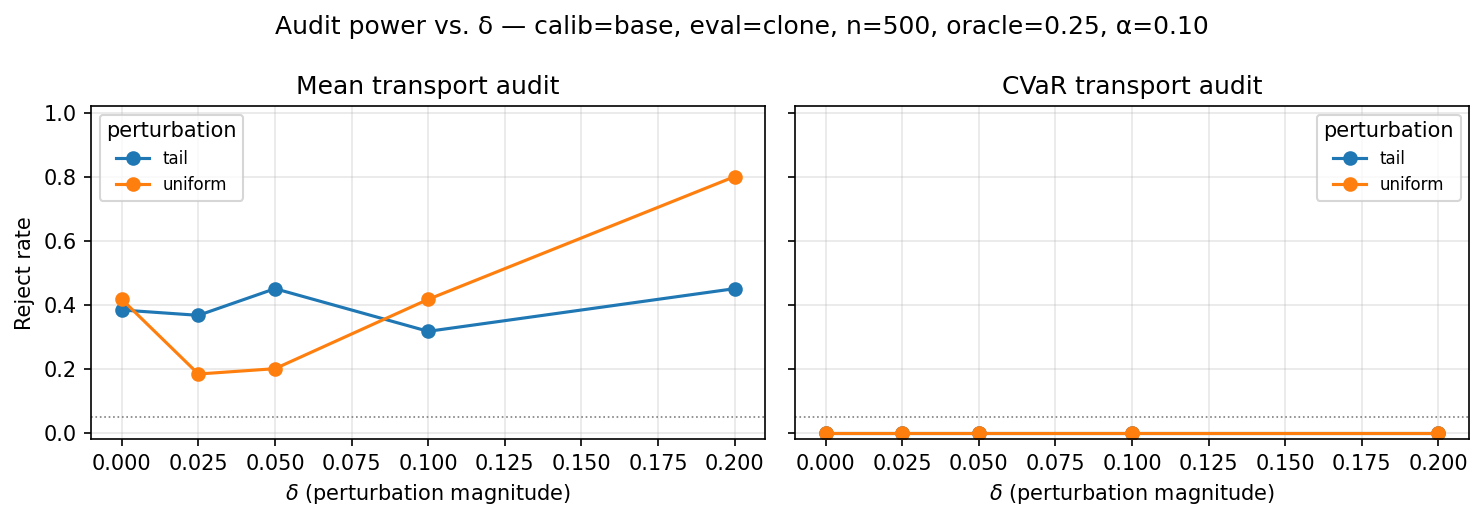
\includegraphics[width=0.92\textwidth]{figs/mc_validation_power_curve.png}
  \caption{\textbf{Audit power curves.} Reject rate vs.\ perturbation
    magnitude $\delta$ for the Mean transport audit (left) and the
    cross-fit two-moment CVaR audit (right). Dotted line marks the
    nominal $0.05$ size. The Mean audit gains power against the uniform
    perturbation as $\delta$ grows but is largely insensitive to the
    tail-only perturbation, as expected for a global-moment test. The
    CVaR audit registers $0$ rejects across the sweep — the bootstrap
    covariance ridge dominates at the production audit-slice size, so the
    audit cannot detect any of the perturbations. We treat this as a
    finding about the audit's small-sample regime, not a property of
    transport.}
  \label{fig:mc-validation-power-curve}
\end{figure}

\paragraph{Caveats and scope.}
\begin{itemize}[leftmargin=*,nosep]
  \item \textit{Estimator scope.} The MC validates the headline pipeline:
    single-stage isotonic calibrator (no length covariate), $\Var_{\text{eval}}$
    from bootstrap, $\Var_{\text{cal}}$ from delete-one-fold jackknife,
    cross-fit two-moment CVaR audit. The two-stage \texttt{$+$cov} mean
    calibrator (\texttt{fit\_two\_stage\_calibrator}) and the augmented
    one-step estimator $\hat V_{\text{aug}}$ are present in the codebase but
    are not validated here; they are routed through the same harness in a
    follow-up.
  \item \textit{Cross-policy structure.} The DGP samples each policy
    independently, so the natural correlation $r(\Y_{\text{base}},
    \Y_{\pi'}) \approx 0.6$--$0.8$ observed in HealthBench is not
    preserved. The estimator is per-policy in production, so this affects
    only the precision of the truth Monte Carlo, not the validity of the
    coverage claim.
  \item \textit{$Y$ marginal and noise heterogeneity.} The
    $m_{\text{override}} = \hat m_{\text{base}}$ knob makes the
    \emph{conditional mean} of $\Sscore | \Y$ match \texttt{base}'s, but the
    target's $\Y$ marginal and quartile $\sigma$ remain its own. Even at
    $\delta{=}0$, this leaves real per-policy mis-specification that the
    calibrator must transport across — and the audit must catch when it
    cannot. The MC results therefore measure inference machinery and
    transport stress jointly; the \texttt{base $\to$ base} cell isolates
    the inference machinery alone.
  \item \textit{Sample sizes.} Coverage cells go up to $n{=}500$ (matching
    the production pilot); we did not extend to $n{=}5000$ because the
    HealthBench production data is bounded above by the actual prompt
    panel size. The trend in $n$ across cells is monotone toward better
    coverage, which is the qualitative validation we need from this study.
\end{itemize}

\paragraph{Takeaway.}
At the production cell ($n{=}500$, oracle coverage $0.25$,
$\alpha{=}0.10$, uniform design), the appendix surfaces three concrete
issues that the headline pilot table on real HealthBench data inherits:

\begin{enumerate}[leftmargin=*,nosep]
  \item \textbf{Mean-CJE coverage is nominal on transport-friendly policies
    (\texttt{base}, \texttt{clone}) and drops sharply on policies whose
    $\Y$ marginal differs from the logger's} — to $0.37$--$0.57$ for
    \texttt{premium}, \texttt{parallel\_universe\_prompt},
    \texttt{risky}, and \texttt{unhelpful}. The Mean transport audit
    correctly flags the same policies; per-policy claims should be gated
    by it.
  \item \textbf{CVaR-CJE coverage is uniformly below nominal at
    $\alpha{=}0.10$} ($0.61$--$0.82$ across policies) because the
    saddle-point estimator's atom-split bias is not absorbed by the
    percentile bootstrap. Coverage rises substantially at $\alpha{=}0.30$
    (looser tail). The full-pipeline bootstrap
    (\texttt{pipeline\_bootstrap\_cvar} in
    \texttt{cvar\_v4/eda/deeper/\_estimator.py}) is the next step toward
    closing this gap; routing it onto the headline path is a tracked
    work item.
  \item \textbf{The cross-fit two-moment CVaR audit has no detectable
    power at production audit-slice sizes ($n_{\text{audit}}{\sim}125$)}
    because the bootstrap-covariance ridge dominates the moment variance.
    Practitioners should not gate CVaR claims on this audit alone at
    production scale; a larger oracle slice, or a re-derived variance
    estimator without the ridge floor, are the natural follow-ups.
\end{enumerate}

We treat the appendix as an accountability ledger, not a victory lap: the
numbers in \cref{tab:mc-validation-headline} and
\cref{tab:mc-validation-power} are the reference any future change to the
estimator stack should improve on, with \texttt{cvar\_v4/eda/deeper/mc\_validation/tests.py}
as the regression gate.
